\chapter{Accessibility}
\label{ch:accessibility}
% ##################################################################################################################

\hfill \textbf{Author:} Dominik Ziemke

\begin{center} 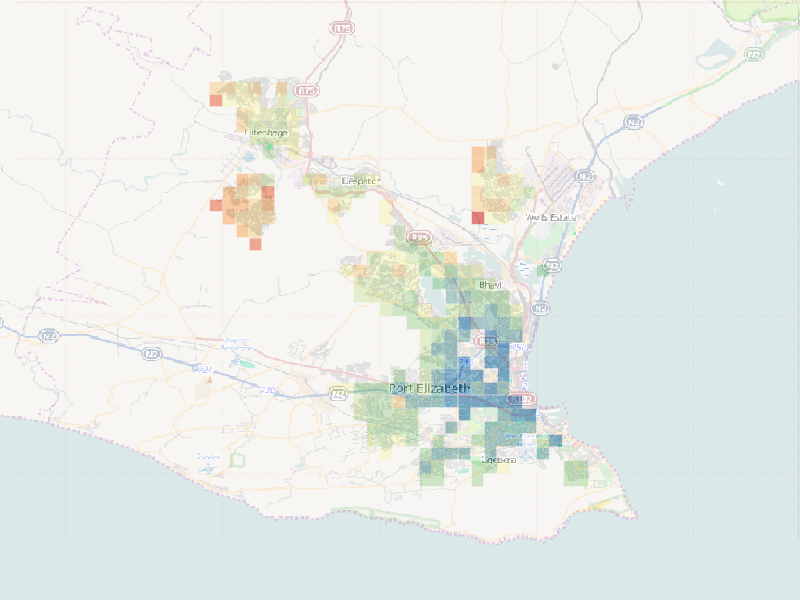
\includegraphics[width=0.5\textwidth, angle=0]{extending/figures/accessibility/w_freeSpeed_snapshot.png} \end{center}

\editdone{This text has undergone the professional edit. Please no grammatical changes anymore! They are most-probably wrong.}

\createStandardInformation{accessibility}{\lstinline{RunAccessibilityExample} class}{accessibility}{\citet{NicolaiNagelHiResAccessibilityMethod}}

% ##################################################################################################################
%\mnote{wider context}
In transport science and planning, the term accessibility can refer to at least three different concepts. 
First, accessibility may be used to describe how well a certain transport infrastructure component 
can be utilized by travelers, particularly those with handicaps \citep{Faura2012AccessibilityEvaluationTrafficSimulation}. 
In this sense, \emph{accessibility guidelines} tell engineers and planners how to design transport 
infrastructure elements, such as public transport facilities, to make them accessible, \ie useable 
for all travelers. Second, accessibility may be used to describe how easy/convenient the approach 
to a given land-use facility is. There are, for instance, studies \citep{Fujiyama2004AccessibleDesignPTFacilities} 
to improve the accessibility of shopping centers by redesigning access roads and their 
connection to major roads. Finally, the term accessibility can be used in a more global way, to 
describe availability and spatial distribution of activity facilities within a given area, \eg a 
metropolitan region and the ease with which these facilities can be reached from other locations in
the area. \gls{matsim}'s accessibility extension focuses on all these aspects; 
the discussion in this chapter draws on \citet{NicolaiNagelHiResAccessibilityMethod}.

% ##################################################################################################################
\section{Introduction}
Improvement in accessibility is often defined as a central goal of proposed transport or infrastructure 
schemes \citep{GeursEtAl2012AccessibilityTransportIntroduction} and 
accessibility is usually a precisely-defined, quantitative measure. While 
\citet{Batty2009AccessibilityUnifiedTheory} traces the origins of the accessibility concept back to 
location theory and regional economic planning in the 1920s (when transport planning began in North America)
\citep{GeursEtAl2012AccessibilityTransportIntroduction}, 
Hansen, with his widely-cited paper \citep{Hansen1959HowAccessibilityShapesLandUse}, is generally credited 
with the first real definition of accessibility, defining it  
as \emph{the potential of opportunities for interaction} 
%also said so e.g. in Gulhan p.130
In more detail, \citet{MorrisEtAl1979AccessibilityIndicators} define accessibility as ``the ease with 
which activities may be reached from a given location using a particular transportation system''.
%\citet{DalviMartin1976MeasurementAccessibility} define accessibility as 'the ease with which any 
%land-use activity can be reached from a location using a particular transport system'. 
% I (dz) I think the above citation is wrong; read this somewhere, but dont know anymore where it was
The concept of accessibility is a potential methodology for the assessment 
of transport systems, as it is a comprehensive and inclusive way to evaluate how, where and why 
people move, taking well-known dependencies between transport and land use into account.
\citet{Hansen1959HowAccessibilityShapesLandUse} was probably the first to develop a procedure for 
quantitative consideration of accessibility, discussed in more detail in Section~\ref{sec:potential}.

%MorrisEtAl1979AccessibilityIndicators, p.92
%accessibility indicators provide possibly the most useful and appropriate means of summarising a great deal of 
%information on the location of households in relation to the distribution of urban activities and the transport 
%system that connects them (Wachs 1978)

%CurtisEtAl2013AccessibilityPolicyInnovation, p.471, definition:
%Accessibility here is defined as the ease or convenience of reaching a destination and is measured by the number 
%of people with access to certain land-use activities or facilities (opportunities) as well as to the transport 
%network itself. This is different to the way some conceive accessibility where it has been used in relation to 
%the mobility needs of elderly or disabled populations (universal accessibility).

%from ERAfrica proposal
%The term “accessibility” has recently gained attention as a potential alternative and state-of-the-art metric as 
%it is a more comprehensive and inclusive way to evaluate how, where and why people move. Accessibility focuses 
%less on the quality and quantity of travel, and more on the needs of households and individuals. Axhausen et al (2011) 
%highlight that accessibility requires knowledge of the activity opportunities for the population, the population 
%characteristics itself, and the generalized cost of travel between activities. With generalized cost we mean the 
%sum of monetary and non-monetary costs. Definitions by Bocarejo and Oviedo (2012), Knowles (2009) and Litman 
%(2010) all emphasize the ease with which individuals have access to goods, services, employment, education, etc. 
%Litman (2010) refers to these activity types, that individuals wish to participate in, collectively as opportunities. 
%Other definitions focus on the mere ability to access opportunities, as opposed to the ease of access (Fan and 
%Huang, 2011; Gutirrez, 2009). In contrast to access, which measures the cost of reaching one particular location 
%and opportunity, accessibility measures the set of all potentially reachable opportunities and is in this way, a 
%measure of total quality of a location as a starting place from the point of view of a traveller. Adopting the 
%point of view of a supplier accessibility measures the potential in terms of visitors or customers to that location 
%as a destination.

%BuettnerEtAl2010Erreichbarkeitsatlas, p.43
%Erreichbarkeit ist **keine** eindeutig definierte Größe. Stattdessen wurden über die letzten Jahrzehnte 
%verschiedene Ansatze zur Quantifizierung des schwer fassbaren Erreichbarkeitsbegriffs entwickelt. Eine 
%weitreichende Einigkeit herrscht in der Wissenschaft allerdings darüber, dass sich Erreichbarkeitsindikatoren 
%durch die Eigenschaft auszeichnen, Merkmale der Siedlungsstruktur einerseits und des Verkehrsangebots 
%andererseits zusammenzuführen


%\mnote{typology}
%Depending on the concrete definition of quantitative accessibility measures, the explanatory power of the 
%result varies widely. As pointed out by \citet{GeursRitsema2001AccessibilityMeasures} (\citep[see also][]{Geurs2004AccessibilityReview}), quantitative indicators can rely on the following approaches:
In their widely-cited review, \citet{Geurs2004AccessibilityReview} identify four accessibility components 
from existing definitions and applied measures:

\begin{enumerate}\styleEnumerate
	\item The \imp{land-use} component reflects
	the number and spatial distribution of opportunities.
	
	\item The \imp{transport} component describes the effort
	to travel from a given origin to a given destination.
	
	\item The \imp{temporal} component considers the availability of activities at
	different times of day, \eg during morning peak hours.
	
	\item The \imp{individual} component addresses various socio-economic groups' different needs and
	opportunities, \eg different income groups.
\end{enumerate}

%\begin{enumerate}
%\item An \textbf{activity-based} or \textbf{land-use-based} approach focuses on
%the distribution of possible activity locations (land use). One can, for instance,
%base calculations on the number and spatial distribution of activity opportunities
%like shopping locations or workplaces within a certain distance.
%%
%\item An \textbf{in\-fra\-struc\-ture-based} or \textbf{transport-based} approach takes into account the effort 
%to travel from a given origin to a given destination and 
%can be based on performance characteristics of the transport system, e.g. the
%average speed by mode at certain locations. If one considers, for instance, the
%number of shopping locations or workplaces under a defined travel time threshold,
%the activity-based and the infrastructure-based approaches can be combined.
%%
%\item A \textbf{temporal} component, which considers the availability of activities at
%different times-of-day, may be added.
%%
%\item An \textbf{individual} approach to accessibility computations can be
%obtained by addressing different needs and opportunities of different socio-economic groups, \eg different income groups.
%%
%\item A \textbf{utility-based} measurement of accessibility reflects the
%(economic) benefits, as the maximum expected utility, that someone gains
%from access to spatially distributed opportunities
%\citep{GeursRitsema2001AccessibilityMeasures,deJongEtAl2007LogsumTRA}. The
%typical example is the logsum term, which is discussed further below.
%\end{enumerate}

In this review, \citet{Geurs2004AccessibilityReview} list and summarize typical approaches applying the accessibility concept, 
focusing on the accessibility components discussed above:

\begin{enumerate}\styleEnumerate
	\item \imp{Infrastructure-based} measures focus on the (observed or simulated) performance or service level 
	of transport infrastructure, \eg represented as average travel speed. These measures are typically used 
	in transport planning.
	
	\item \imp{Location-based} measures describe level of accessibility to spatially distributed activities, such as 
	 number of jobs within 30\,minutes travel time from origin locations. These measures are typically used 
	in urban planning and geographical studies.
	
	%CurtisEtAl2013AccessibilityPolicyInnovation, p.456
	%Activity- or destination-based accessibility modelling has expanded rapidly with the coalescing of advanced GIS
	
	\item \imp{Person-based} measures analyze accessibility at the individual level, such as the activities in which an 
	individual can participate at a given time. These measures are grounded in \citet{Haegerstrand1970WhatAboutPeople}'s space–time geography.
	
	\item \imp{Utility-based} measures analyze the economic benefits that people derive from access to spatially 
	distributed activities. These measures have their origin in economic studies.
\end{enumerate}

\citet{Geurs2004AccessibilityReview} intersects these approaches with the four accessibility components identified 
above, creating a matrix. This matrix illustrates how each of the four accessibility components is 
 represented in the four different accessibility measures. There, each measure focuses on certain weaknesses 
in those accessibility components outside the focus of a specific measure. Accordingly, \citet{Geurs2004AccessibilityReview} recommend that an accessibility measure include all four discussed accessibility components. The accessibility extension of \gls{matsim}, described in 
the following, could be one way to achieve this goal.

%\mnote{latest research}
In other recent research, as identified by \citet{GeursEtAl2012AccessibilityTransportIntroduction},
the accessibility concept is also applied to social exclusion analysis (\eg by examining the benefit of
employment accessibility for disadvantaged populations before and after the implementation of a 
transport scheme), economic valuation of accessibility effects (\eg in cost-benefit analyses and studies 
assessing the impact of changes in public transport accessibility on house prices) and behavior analysis 
vis-a-vis accessibility measures (\eg walking behavior dependence on different residential neighborhood accessibility qualities).
It has also been used to explore questions of oil dependence, climate change and 
other concerns \citep{CurtisEtAl2013AccessibilityPolicyInnovation}.

%CurtisEtAl2013AccessibilityPolicyInnovation, p.455f
%New forms of transport analysis are emerging that can be used, in addition to the traditional transport models, 
%to expand knowledge and enable a fuller range of policy issues to be examined. Advances in the rise of geographic 
%information systems (GIS) has allowed for new methods to explore questions of equity and access (Halden, 2002), oil 
%vulnerability (Dodson and Sipe, 2007), climate change (Hickman et al., 2010) and other emergent concerns. Activity- or 
%destination-based ac- cessibility modelling has expanded rapidly with the coalescing of advanced GIS, comprehensive 
%spatial datasets, exemplar projects and skills development in the planning and transport professions

%MorrisEtAl1979AccessibilityIndicators, p.92
%The two principal bases of classification are the behavioural dimension mentioned earlier, and a dis- tinction between 
%“relative accessibility” and “ integral accessibility” developed by Ingram (1971). Relative accessibility describes the 
%relation or degree of connection between any two points, whereas integral accessibility describes the relation or-degree 
%of interconnection be- tween a given point and all others within a spatial set of pointst (see Fig. 2.)

% ##################################################################################################################
\section{The Measure of Potential Accessibility}
\label{sec:potential}
%\mnote{measures in practice}
Today, methods to assess accessibility quality are often used in superordinate planning procedures, like 
regional transport planning, where a central goal is to provide citizens with a certain level of access to
various services. For instance, the approach used by Germany's agency responsible for regional planning calculates
travel times to major service facilities, like airports or hospitals \citep{BBSRErreichbarkeitsmodell}. The results,
typically visualized by multi-colored maps, give useful insights 
into population access to certain services, thus aiding transport 
infrastructure planning.
% transport component
% As such, this definition of an accessibility measure has its focus on the \textbf{trasnport component} of accessibility 
% as introduced above.
In this approach, travel times are calculated to an \emph{next} airport, \emph{next} hospital and
 \emph{next} autobahn access; thus, the implicit assumption is that citizens' needs are fulfilled by
one (\ie the \emph{next}, or closest in terms of travel times) type of facility.

%BuettnerWulfhorstEtAl2013Vulnerability, p.13
%given number of jobs accessible by a given mode of transport (here: public transport) within a given amount of time (here: 
%60min) displayed in a colored my by municiplaity, i.e. on a zone-based level; data source: Erreichbarkeitsatlas
%BuettnerWulfhorstEtAl2013Vulnerability, p.14
%basically the same for Lyon: Isochrone accessibility to jobs is measured for public transport commuters, in the morning 
%peak period. Travel time is computed using a “shortest path algorithm”

%\mnote{land-use component}
An accessibility measure becomes significant, however, if not just the ability to reach \emph{the nearest} facility 
serving a particular need is taken into account, but also a \emph{set of multiple reachable} facilities serving the same 
need; different facilities of the same type may offer varying qualities of a given service. 
Services may also expand and improve when combined with complementary services provided by 
another facilities of the same type. For instance, a person planning to take a holiday trip by plane will probably 
consider several airports in his/her vicinity, instead of just looking at flights 
offered from the nearest airport. Thus, accessibility to airports should be made dependent on the ability 
to reach all local airports instead of just the nearest one. Facilities offering medical 
services may serve as another example. Considering the nearest hospital may be sufficient when looking 
at simple services like first aid, presumably available at almost \emph{any} hospital. In other cases, 
however, medical services accessibility should consider several hospitals in the vicinity 
because they are likely to offer different specialized medical treatment.
%\Karen{Please check the meaning of this last sentence; I did not feel it made sense in the original version.  Thanks!} 
%\ah{adapted according to my understanding}
% land-use componenent
Consideration of a set of multiple facilities, potentially useful from the perspective of a person at
a given location, corresponds to 
%respecting 
%\Karen{What does "respecting" mean here? I don't get it, sorry.  Thanks.}
taking into account the \imp{land-use component} of accessibility defined above.

%\mnote{potential accessibility}
Hansen's early study \citep{Hansen1959HowAccessibilityShapesLandUse} 
considers the whole scope of potential activity facilities, where an accessibility 
measure \emph{potential accessibility} is defined. Such measures of potential accessibility are 
specified as the (weighted) sum over the 
accessibilities of several specific activity facilities (\eg shopping, leisure etc.) and take the mathematical form
%The (quantitative) accessibility measure in the MATSim accessibility extension is of the mathematical form
\begin{equation}
	%A_i = g\Big( \sum_j a_j \, f(c_{ij}) \Big) \ ,
	A_\ell = g\Big( \sum_j a_j \, f(c_{\ell j}) \Big) \ ,
	\label{eq:accessibility:basic}
\end{equation}
%\kai{Ein Problem(chen) hier ist, dass wir im Buch $i$ als den ``index of selected alternative'' haben.  Sollten wir in diesem Kapitel noch $i$ durch $\ell$ (für ``location'') ersetzen?}
%where the sum goes over all possible destinations (opportunities) $j$, $a_j$ is an indicator of the attractiveness of 
%the opportunity, $c_{ij}$ is the generalized cost of travel to get from $i$ to $j$, $f(c)$ is an impedance function 
%that typically decreases with increasing distance, and $g(.)$ is an arbitrary, but typically monotonically increasing, 
%function. 
where $j$ are all possible destinations (opportunities), $a_j$ describes opportunity attractiveness, 
$j$, $c_{\ell j}$ denotes the generalized traveling cost between origin $\ell$ and destination $j$,
$f(c)$ is an impedance function which (typically) decreases with increasing distance and $g(.)$ denotes
an arbitrary, but usually monotonically increasing function. 
%That is, the accessibility at $i$ is computed from a weighted sum over all possible destinations, where the weight is 
%the product of the destination's attractiveness and the ease to get there.
Weight is the product of the destination's attractiveness and the ease of getting there. As seen in its 
functional form, this type of accessibility measure is related to gravity models used in trip generation models, explaining 
why this measure is sometimes also referred to as a ``gravity type'' accessibility indicator 
\citep{MorrisEtAl1979AccessibilityIndicators}. The (quantitative) accessibility measure used in the \gls{matsim} 
accessibility extension is expressed in this mathematical form and may thus be seen as a \emph{potential accessibility} measure.

%MorrisEtAl1979AccessibilityIndicators, p.94
%the “gravity type” indicators, as introduced by Hansen (1959), lend themselves to a variety of functional forms of 
%impedance (power, exponential, Gaussian, etc.)

%BuettnerEtAl2010Erreichbarkeitsatlas, p.44
%Die methodische Grundidee der ortsbezogenen Erreichbarkeitsindikatoren liegt darin, dass ein Ausgangsstandort
%mit allen gegebenen Zielstandorten bzw. Teilraumen innerhalb des definierten Untersuchungsgebiets in Beziehung 
%gesetzt wird. Jedem Ziel- standort ist ein Potenzial zugeordnet. Die Summe dieser Potenziale ist die Erreichbarkeit 
%des Ausgangsstandorts. Das Potenzial eines Zielstandorts wird dabei in der Regel durch die strukturelle Große dieses 
%Standorts definiert (z.B. Einwohnerzahl, Verkaufsflache). Allerdings wird in Abhängigkeit des Raumwiderstands 
%(Reisezeit, Kosten etc.), der für die Reise vom Ausgangs- zum Zielstandort überwunden werden muss, eine Abwertung 
%des Potenzials vorgenommen.

%\mnote{ingoing vs. outgoing accessibility}
It is important to note that the above-defined measure quantifies how accessible a given location is \emph{to} certain
services $\ell$. This kind of accessibility is \emph{outgoing accessibility},
while a measure of \emph{ingoing accessibility} quantifies how accessible a given
destination location $j$ is \emph{from} other locations. \citet{NicolaiNagelHiResAccessibilityMethod} 
discuss circumstances under which these measures are interchangeable.

% ##################################################################################################################
\section{Accessibility Computation integrated with Transport Simulation}
\label{sec:integrated}
%\mnote{transport component}
%\mnote{uncongested vs. congested network}
As mentioned above, accessibility computations are often based on travel times 
\citep{BBSRErreichbarkeitsmodell, BuettnerEtAl2010Erreichbarkeitsatlas}, which serve as an impedance measure.
Ways of calculating these travel times can, however, vary significantly. 
The simplest way to calculate a travel time between two locations is to measure the Euclidean distance 
(beeline distance) between these two locations and then, by averaging speed, approximate the 
travel time between them. According to \citet{Geurs2004AccessibilityReview}, this is the usual 
approach in location-, person-, and utility-based accessibility approaches, where the focus 
is not specifically on the transport system.

%CurtisEtAl2013AccessibilityPolicyInnovation, p.458
%This led to the development of an impediment measure based on properties most closely related to users’ experience: 
%that is, travel time, journey transfer and frequency of service, rather than geographical distance.

%BuettnerEtAl2010Erreichbarkeitsatlas, p.49
%Erreichbarkeit berechnet sich gemaß des dargestellten Konzepts einerseits aus den Potenzialen, der im Untersuchungsgebiet 
%liegenden Standorte (dies konnen z.B. Verkehrszellen sein) sowie andererseits aus den Widerständen der Raumuberwindung, 
%welcher der Einfachheit halber meist durch die Reisezeiten abgebildet werden

To strengthen the \imp{transport component} of accessibility (as introduced above) and 
make accessibility measure sensitive to transport infrastructure changes, a better representation of the travel 
impedance between origins and destinations is required. The most common approach is be travel time calculation
using shortest-path algorithms on a real-world transport infrastructure network representation.
Many accessibility computations are embedded into \gls{gis} software, offering procedures for network-based 
computations 
\citep{BBSRErreichbarkeitsmodell, CurtisEtAl2013AccessibilityPolicyInnovation, BuettnerEtAl2010Erreichbarkeitsatlas}.

%CurtisEtAl2013AccessibilityPolicyInnovation, p.458
%SNAMUTS is a GIS-based tool designed to measure the accessibility provided by existing or proposed urban public transport networks
%
%CurtisEtAl2013AccessibilityPolicyInnovation, p.466
%The model is essentially a destination-based accessibility model run using ArcGIS software

The accessibility extension in \gls{matsim} also offers this type of accessibility computation. To run it, an 
accessibility controler listener, \eg the \lstinline{GridBasedAccessibilityControlerListenerV3} must be added to 
the \gls{matsim} controler. An example is given in \lstinline{RunAccessibilityExample} (see
\url{http://matsim.org/javadoc} $\to$ accessibility $\to$ \lstinline{RunAccessibilityExample} for details). As input, a 
network file and facilities file are required (for more information on networks and facilities, refer to 
Section~\ref{sec:using-network} and Section~\ref{sec:extending-facilities} of this book).
This procedure is more disaggregate than many common approaches to accessibility computations, where single 
facilities are seldom considered; there, structural data like zone sizes, number of jobs, or total sales area are used to 
represent the \emph{potential} of a given zone 
\citep{BuettnerEtAl2010Erreichbarkeitsatlas, GulhanEtAl2014PotentialAccessibilityMeasureDenizli} (also see
Section~\ref{sec:spatial}).

%sales area = Verkaufsraumfläche

%\mnote{demand/supply effects - effects of competition}
Either way, performing an accessibility computation this way can be regarded as a \emph{supply-based approach}, 
since both supply with transport infrastructure (required to reach a given location) and supply with 
activity opportunities at these locations are taken into account. The utilization of these two supply dimension by users, 
\ie the dimension of \emph{demand} is, however, not considered in this approach. Therefore, no 
\emph{effects of competition} \citep{Geurs2004AccessibilityReview}, either for transport infrastructure resources 
(defined by network capacities), or activity facilities capacities, are taken into account. It is 
obvious, however, that supply and demand interaction effects are relevant, because opportunities may disappear 
if they can no longer be reached within reasonable travel times, or when activity facility capacities 
are exceeded. 

%\mnote{advantages over GIS-based tools}
By considering demand-supply interaction effects in addition to just the
supply side, the scope of the accessibility calculation can be significantly increased.
Gauging these effects on \emph{facility capacities} can be addressed by specifying facility
capacities in the according value in the \lstinline{facilities} input file. The corresponding code adaption for
observing these capacities in the \gls{matsim} accessibility extension is currently underway. Observation of
\emph{network capacities} and their effects on agents' behavior, by contrast, is one of the core features
of the \gls{matsim} transport simulation. This is also one major argument for the integration of an accessibility
computation with the dynamic transport simulation system \gls{matsim}. While other accessibility tools, (the
majority based on \gls{gis} systems
\citep{BBSRErreichbarkeitsmodell, CurtisEtAl2013AccessibilityPolicyInnovation, BuettnerEtAl2010Erreichbarkeitsatlas, LiuZhu2004AccessibilityAnalyst, GulhanEtAl2014PotentialAccessibilityMeasureDenizli})
can calculate travel times on a routed network, they do not calculate accessibilities dependent on transport infrastructure usage
level. This property, is, however, essential when making accessibility measures sensitive to
transport demand management policies, \ie transport system changes that do not alter the transport
infrastructure and are thus not captured by models considering only the supply side.

%BuettnerEtAl2010Erreichbarkeitsatlas, p.49
%Die Erreichbarkeitsatlas-Datenbasis wurde im Wesentlichen auf der Sofware-Plattform ESRI ArcGIS (Version 9.2) aufgebaut. 
%Dies gilt fur alle raumlichen Strukturdaten sowie fur die Verkehrsangebotsdaten des Individualverkehrs. Einzig das 
%Angebotsmodell des offentlichen Verkehrs wurde nicht auf GIS-Basis, sondern auf Basis der VISUM Verkehrsmodellplattform 
%(Version 10) der ptv AG erstellt (vgl. Kap. 3.4.3.2). Die Berechnung der Erreichbarkeitsindikatoren erfolgt mit Microsoft Excel 2007.

To take these effects into account, the \gls{matsim} accessibility extension must be run with a \gls{matsim} 
transport simulation. To do so, an initial plans file (as described in Chapter~\ref{ch:lgstarted} of this book) 
needs to be specified in the \gls{matsim} \gls{configfile}. Furthermore, the value \lstinline{timeOfDay} in
the \lstinline{accessibility} module of the \gls{matsim} \gls{configfile} needs to be specified. If then, as 
described, an accessibility controler listener is added to the \gls{matsim} controler, the best-path travel
times, on which the accessibility computation will be performed, are taken from travel times observed in
the \gls{matsim} transport simulation at the time specified by the value \lstinline{timeOfDay}. This is useful 
when transport demand level varies significantly during the day; for instance, 
with morning and afternoon peaks; it also allows transport policy accessibility changes 
(and decision makers' reactions) to be better analyzed.
%which would appears cumbersome in 
%cases where the accessibility computation is not coupled with a dynamic traffic simulation.

% ##################################################################################################################
\section{Econometric Interpretation}
%\mnote{econometric interpretation} 
As pointed out by \citet{MorrisEtAl1979AccessibilityIndicators}, accessibility indicators provide a very
useful way to summarize a large volume of information on household locations and how they relate to 
urban activities' distribution and connecting transport systems.
%
%MorrisEtAl1979AccessibilityIndicators, p.92
%accessibility indicators provide possibly the most useful and appropriate means of summarising a great deal of 
%information on the location of households in relation to the distribution of urban activities and the transport 
%system that connects them (Wachs 1978)
%
They also take land use, the transport system and their inter-dependencies into
account holistically.
%
%the well-known transport-land-use cycle that describes the bidirectional interrelationship between transport and land use
%
\citet{CurtisEtAl2013AccessibilityPolicyInnovation} explain that accessibility assessment tools overcome
policy innovation restrictions associated with traditional transport planning practice, pointing out that use of
such tools enables examination of a broader range of policy issues.

% explicitly observes the interrelationship between transport and land use.

%
%CurtisEtAl2013AccessibilityPolicyInnovation, p.454
%New accessibility tools offer the possibility to guide these policy changes, overcoming restrictions to policy innovation associated with traditional transport planning practice.
%
%CurtisEtAl2013AccessibilityPolicyInnovation, p.454
%absence of planning support tools that can inform decision-making about public transport networks
%
%CurtisEtAl2013AccessibilityPolicyInnovation, p.455f
%New forms of transport analysis are emerging that can be used, in addition to the traditional transport models, 
%to expand knowledge and enable a fuller range of policy issues to be examined. Advances in the rise of geographic 
%information systems (GIS) has allowed for new methods to explore questions of equity and access (Halden, 2002), oil 
%vulnerability (Dodson and Sipe, 2007), climate change (Hickman et al., 2010) and other emergent concerns. Activity- or 
%destination-based ac- cessibility modelling has expanded rapidly with the coalescing of advanced GIS, comprehensive 
%spatial datasets, exemplar projects and skills development in the planning and transport professions
%
%CurtisEtAl2013AccessibilityPolicyInnovation, p. 455
%Public-transport focused accessibility models are also becoming more common.
%
%CurtisEtAl2013AccessibilityPolicyInnovation, p.455
%While these new tools, like the traditional transport models, sit within a positivist framework, they expand the field of
%positivist analysis in new directions. They also rely on a logical and mathematical treatment to provide scientific knowledge
%
%CurtisEtAl2013AccessibilityPolicyInnovation, p.455
%The application of each tool has intersected with transport and land-use decision-making, attempting to reveal
%insights that would influence decision-makers to consider alternative transport futures

For effective policy decisions, accessibility assessment tools must be economically interpretable.
To make an accessibility measure clearest in an econometric evaluation (\eg cost-benefit 
analyses), it seems sensible to adapt equation \ref{eq:accessibility:basic} as 
%follows: $g(.) = \ln(.)$, $a_j = 1$, $f(c_{ij}) = e^{-c_{ij}}$, and $-c_{ij} = V_{ij}$. Thus, 
follows: $g(.) = \ln(.)$, $a_j = 1$, $f(c_{\ell j}) = e^{-c_{\ell j}}$, and $-c_{\ell j} = V_{\ell j}$. Thus, 
equation \ref{eq:accessibility:basic} becomes
\begin{equation}
	%A_i := \ln \sum_k e^{V_{ik}} \ ,
	A_\ell := \ln \sum_k e^{V_{\ell k}} \ ,
	\label{eq:accessibility:logsum}
\end{equation}
where $k$ denotes all possible destinations and $V_{\ell k}$ equals the disutility of traveling from location $\ell$
to destination $k$. Equation~(\ref{eq:accessibility:logsum0}) is the so-called \gls{logsum} term and can be interpreted
as the expected maximum utility \citep[e.g.,][]{BenAkivaLerman_1985, DejongEtc2005LogsumAsEvalDutchReport}. Equation
\ref{eq:accessibility:logsum} can be derived by assuming that the full utility of destination location $k$ as
perceived at origin location $\ell$, is $U_{\ell k} = V_{base} + V_{\ell k} + \epsilon_{\ell k}$,
where $V_{base}$ is a base utility for performing a given activity without considering its location,
$V_{\ell k}$ is the systematic or observed disutility of traveling to from origin $\ell$ to destination $k$,
and $\epsilon_{\ell k}$ is a random term which absorbs the randomness of disutility of traveling, as well as
fluctuations in utility around $V_{base}$. Under the usual assumption that the $\epsilon_{\ell k}$ are
independent and identically (iid) Gumbel-distributed random variables, the expectation value of $U_{\ell k}$ becomes
\begin{equation}
	%E(U_i) = E(\max_k U_{ik}) = \ln \sum_k e^{V_{ik}} + Const \equiv A_i + Const \ .
	E(U_\ell) = E(\max_k U_{\ell k}) = \ln \sum_k e^{V_{\ell k}} + Const \equiv A_\ell + Const \ .
\end{equation}
$Const$ does not need to be considered, as it is invariant for all locations. $A_\ell$ may, therefore, also
take negative values.

\citet{GeursEtAl2012AccessibilityBenefitsNetherlands}, for instance, use the \gls{logsum} measure of user benefits 
as an alternative to the travel time savings method (\ie rule-of-half measure) in a case study 
examining the effects of spatial planning on accessibility benefits and economic efficiency of public 
transport projects.

%In Chapter 8, Karst T. Geurs, Michiel de Bok and Barry Zondag examine the degree to which spatial planning affects 
%the accessibility benefits and economic efficiency of public transport projects. As a case study, plans for a large 
%urban planning project in the Netherlands are examined, combined with major rail investment alternatives (involving 
%the upgrade of an existing bridges and construction of new bridges). The authors apply the logsum measure of user 
%benefits, as an alternative to the travel time savings method (i.e. rule-of-half measure)

%the major disadvantages of utility-based measures are the difficult interpretability and communicability (Geurs p136)

% ##################################################################################################################
\section{Spatial Resolution, Data, and Computational Aspects}
\label{sec:spatial}
%\mnote{spatial resolution, zones vs. points}
In contrast to many other transport simulations, \gls{matsim} is based on coordinates (see Chapter~\ref{ch:lgstarted} of this book),
not zone-based.
Therefore, accessibility computation in \gls{matsim} can also
be conducted independent  from any zoning system and, instead, be based on a raster with arbitrary granularity,
\ie adjustable grid size. Depending on the calculation planned (zone-based or grid-based), a 
\lstinline{ZoneBasedAccessibilityControlerListenerV3}, or a 
\lstinline{GridBasedAccessibilityControlerListenerV3}, respectively, need to be added to the \gls{matsim} controler 
(See \url{http://matsim.org/javadoc} $\to$ accessibility $\to$ \lstinline{RunAccessibilityExample} for an example
using the \lstinline{GridBasedAccessibilityControlerListenerV3}. More detail about the interpretation
of cell- and zone-based accessibility measures is given in \citet{NicolaiNagelHiResAccessibilityMethod}).
Unlike the \gls{matsim} accessibility extension, most other accessibility assessment tools
rely on the zone-based approach 
\citep{CurtisEtAl2013AccessibilityPolicyInnovation, LiuZhu2004AccessibilityAnalyst, BuettnerEtAl2010Erreichbarkeitsatlas}.
%This is mostly due to a better availability of data at the level of spatial resoultion of a particular zoning system.
Since good quality structural data is only available at certain administrative zone levels, 
\eg municipalities, it is not feasible to conduct these accessibility assessment approaches at a finer 
spatial resolution.

Running a grid-based calculation, especially if a high spatial resolution is selected, avoids several issues
that could arise (like``self-potential'') if accessibility computations are based on zones
\citep[see, e.g.,][]{NicolaiNagelHiResAccessibilityMethod}. A zone-based approach also makes the 
measure dependent on size and shape of the geographical units (\cf \gls{maup}). 
Due to its typically lower resolution level, a zone-based approach may also not adequately represent local details
\citep{Kwan1998PointBasedAccessibility}. This is especially relevant
when lower-speed mode accessibilies (like walking) must be considered.

The \gls{matsim} accessibility calculation does not require typical zone-based statistical data. Instead, the
calculation can be conducted on the basis of so-called \gls{vgi} like \gls{osm}, which contains
activity facilities data on a coordinate-based level. Hence, no reference to any zoning
system is necessary when using these data. Furthermore, data from \gls{osm} is publicly and freely available; 
amount of these data are steadily increasing and quality improving. In particular, \gls{osm} seems to have 
established itself as a uniform and globally-accessible standard for crowd-sourced and other geo-data, 
which makes the \gls{matsim} accessibility assessment highly portable.

%from ERAfrica proposal
%rely on open and freely available data to ensure the use of the metric is duplicable everywhere
%
%from ERAfrica proposal
%A recent advance is that much more input data is now publicly available, often crowd-sourced. Our primary source of 
%open data will be OpenStreetMap (http://osm.org), which seems to have established itself as a uniform and worldwide 
%accessible standard for crowd-sourced and other geo-data. In fact, the use of OpenStreetMap is favoured in the 
%South African environment, the result of strong advocacy for geospatial data to be more readily available for 
%decision-making and decision support. To that extent, the South African National Geospatial Information (NGI) has 
%started to move all its Geospatial Information System (GIS) data over to OpenStreetMap.
%This offers the unprecedented opportunity to bind the new computational methods, outlined above, together with 
%standardized input data. This would make the approach very portable, that is, it could be easily ported to a 
%different spatial location, to the analysis of other types of services, or even a different spatial scale.
%At present, the transportation network information provided by \gls{osm} is already sufficient in most places to 
%obtain plausible results; this holds, in particular, to urbanized locations also in developing countries. The data 
%stock is also growing at an unprecedented pace, so even if input data is not fully available yet it pays off to 
%invest into methods and infrastructure to harvest that data in the near future. Finally, the types of data covered 
%by OpenStreetMap are ever increasing. Concerning pedestrian access in urban areas, it may already be the best 
%global data source around; for example, it contains a full walk network of Kibera in Nairobi which is more than 
%what google maps can feature (accessed 6-Apr-2013). The services to which access should be provided are often 
%already mapped in OpenStreetMap; if not, neighbourhood organizations may map and add these or other service 
%locations to the existing data infrastructure.
%
%from ERAFrica proposal
%Accessibility is conventionally computed for spatial aggregates, such as “zones”, which is problematic in
%particular for situations where walking is an important mode of transport because of its dependence on small 
%scale details. Recent progress on facilities data, network data, transport data, transport modelling, and 
%computational methods has, however, made it possible to compute accessibility measures with very high spatial 
%resolution, if needed down to each individual household location.
%
%from ERAfrica proposal
%Despite the fact that accessibility is a point measure, i.e. a measure that will be different for every 
%coordinate (x,y), it is typically computed for geographical units such as zones or districts. Besides making 
%the measure dependent on the size and shape of the geographical units (“modifiable areas unit problem”, e.g. 
%Openshaw, 1984), this also has the disadvantage of hiding much local detail (e.g. Kwan, 1998), especially when 
%pedestrian accessibility is or should be included. A big obstacle to detailed high resolution accessibility 
%calculations is that the effort to reach a destination should not just use Euclidean distance but should 
%instead be calculated on a detailed transport network, preferably separately for every mode of transport. 
%Kwan (1991) uses a special compute server and still is limited to relatively low resolutions. Advances in 
%hardware and software have, since then, made it feasible to compute high-resolution accessibility in nearly
%arbitrary resolution in acceptable time on standard hardware (NicolaiNagelHiResAccessibilityMethod).
%
%BuettnerEtAl2010Erreichbarkeitsatlas, p.54
%Im Individualverkehr wurde fur den Erreichbarkeitsatlas die Netzdatengrundlage des OpenStreetMap-Projekts 
%gewahlt. Dabei handelt es sich um ein offenes, internet-gestutztes, jedermann zugangliches Kartenprojekt. 
%Die Datenbasis wird durch die Nutzer erstellt und aktualisiert („Wiki-Prinzip‚).
%
%BuettnerEtAl2010Erreichbarkeitsatlas, p.55
%Die Anbindung der Regionalzellen an das OpenStreet-Netzwerk erfolgt zunachst am geometrischen Mittelpunkt 
%einer Zelle. Von diesem aus wird das nachstgelegene Netzelement ermittelt und angebunden. Perspektivisch konnte 
%statt dem geometrischen Mittelpunkt auch – unter Verwendung von Flachennutzungsdaten (vgl. Kapitel 3.5.1.2) – der 
%Nutzungsschwerpunkt ermittelt und die Zelle daruber angebunden werden.

If the coordinate-based ($=$ grid-based $=$ raster-based $=$ cell-based) version of the \gls{matsim} accessibility
computation is selected, its results can be interpreted as an accessibility field, \ie as a measure
that varies continuously in space. This \emph{accessibility field}, can be visualized by calculating
the values on regular grid points. Figure~\ref{fig:accessibility-nmbm} gives an example of such a
visualization and depicts the accessibility of work places in Nelson Mandela Bay Municipality in South
Africa, as calculated by the grid-based \gls{matsim} accessibility computation with a grid size 
of 1\,000\,meters.

%too high computational effort, see below Buettner

%BuettnerEtAl2010Erreichbarkeitsatlas, p.44
%Das Potenzial eines Zielstandorts wird dabei in der Regel durch die strukturelle Große dieses Standorts definiert 
%(z.B. Einwohnerzahl, Verkaufsflache). Allerdings wird in Abhängigkeit des Raumwiderstands (Reisezeit, Kosten etc.), 
%der fur die Reise vom Ausgangs- zum Zielstandort uberwunden werden muss, eine Abwertung des Potenzials vorgenommen.
%
%mention here information from MiD workshop Bonn Fall 2013 where they said that they also plan to use a grid-based spatial
%system in the future

\createfigure%
{Accessibility of work places in Nelson Mandela Bay Municipality calculated
	by the grid-based \gls{matsim} accessibility computation}%
{Accessibility of work places in Nelson Mandela Bay Municipality calculated
	by the grid-based \gls{matsim} accessibility computation}%
{\label{fig:accessibility-nmbm}}%
%{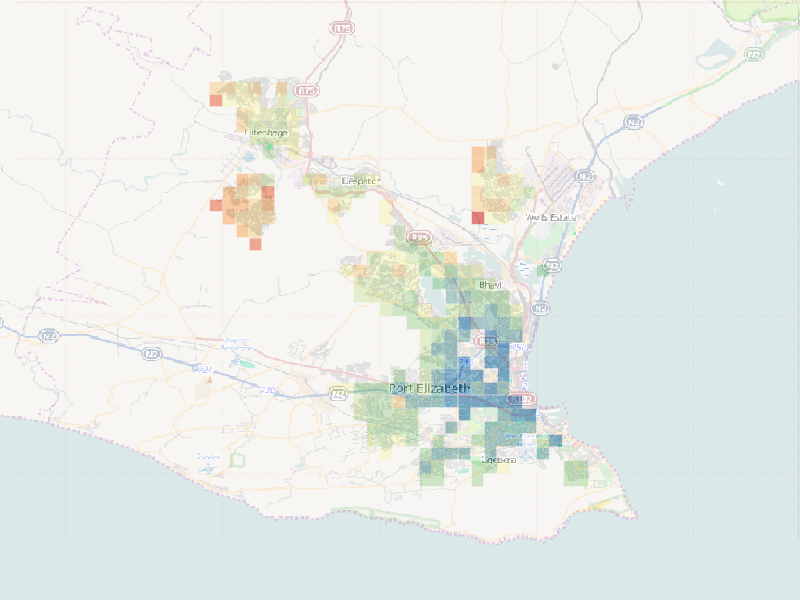
\includegraphics[width=0.99\hsize,trim=2cm 2.5cm 2cm 3cm,clip]{extending/figures/accessibility/w_freeSpeed_snapshot.png}}%
{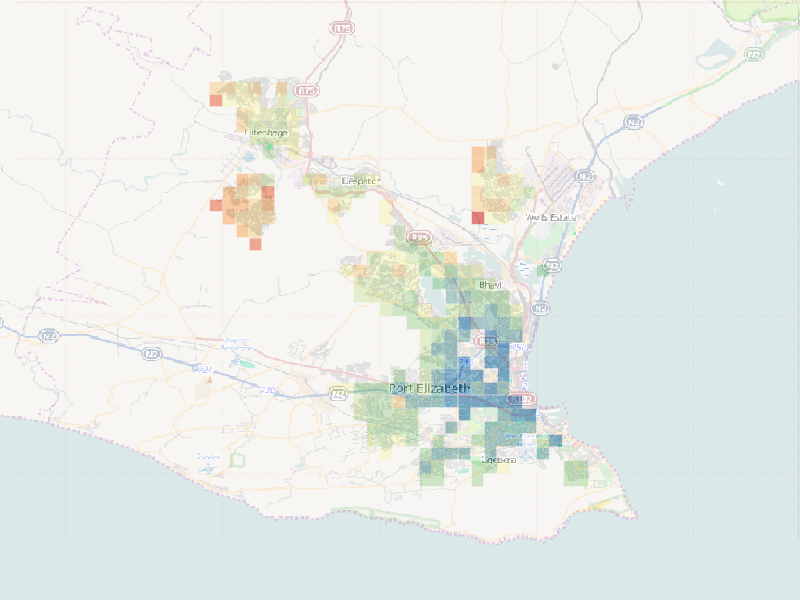
\includegraphics[width=0.99\hsize]{extending/figures/accessibility/w_freeSpeed_snapshot.png}}%
{}

%To use this functionality a \lstinline{GridBasedAccessibilityControllerListenerV3} needs to be added to the controller.
%Alternatively, if the calculation based on some given zonation system is desidered, the 
%\lstinline{ZoneBasedAccessibilityControllerListenerV3} can be used.
%
%BuettnerEtAl2010Erreichbarkeitsatlas, p.49
%Das Raumstrukturmodell stellt im Kern eine Einteilung des Unterschungsgebiets der EMM in kleine Zellen dar. Fur den 
%Erreichbarkeitsatlas wurden zu diesem Zweck die Gemeinden herangezogen, welche auf der Betrachtungsebene der gesamten 
%EMM eine ausreichende raumliche Genauigkeit bieten. Die Gemeinden sind zudem die kleinste raumliche Einheit, fur die
%von Seiten des Statistischen Landesamtes Bayern die benötigten Strukturdaten (z.B. Einwohner- und Beschaftigtenzahlen)
%kostenfrei und einheitlicher Form zur Verfügung gestellt werden.
%
%BuettnerEtAl2010Erreichbarkeitsatlas, p.50
%Erreichbarkeitsmodelle verwenden in der Regel Zellensysteme um raumliche Strukturdaten abzubilden. Der wesentliche Grund
%hierfur ist die große Zahl der einzelnen Datenelemente (z.B. Einwohner, Arbeitsplätze etc.). Wenngleich sich 
%Erreichbarkeitsindikatoren theoretisch auch vollständig disaggregiert berechnen ließen, scheitert dies in der 
%Praxis doch am Rechenaufwand aber auch an der Verfugbarkeit entsprechend feinteiliger Daten. Gangige Praxis ist es 
%deswegen, dass Untersuchungsgebiet in Zellen einzuteilen und die Raumstrukturdaten entsprechend dieser Zellstruktur 
%zusammenzufassen

%\mnote{calculation procedure}
To calculate the accessibility $A_\ell$ of a given origin location $ell$ to opportunity locations $k$, both
the origin location $\ell$, and opportunity locations $k$, are assigned to a road network. If the option to
integrate the accessibility computation with the transport simulation, as described in Section~\ref{sec:integrated},
is chosen, a congested network with time-dependent travel times (as they have been simulated in \gls{matsim})
is used. For every $\ell$, a so-called \emph{least cost path tree} computation
\citep{LefebvreBalmer_unpub_STRC_2007} is carried out. Accessibility of the same location at a different
time of day will usually be different, since congestion patterns vary.
The least cost path tree computation determines the best route and the least negative travel
utility $V_{\ell k}$ from the origin location $\ell$ to each opportunity location $k$, based on Dijkstra's
shortest path algorithm \citep{Dijkstra_NM_1959}. Once the least cost path tree has explored all
nodes, the resulting disutilities $V_{\ell k}$ for all opportunities $k$ are queried and the accessibility
is calculated, as stated in Equation~(\ref{eq:accessibility:logsum}) \citep{NicolaiNagelHiResAccessibilityMethod}.
%
A crucial question is how to choose the point, \ie the coordinate, where the accessibility computation is
anchored. Most quantitative accessibility tools use geographical centroids of given zones. This is also
true when the zone-based \gls{matsim} accessibility computation is selected. Alternative ways to select
a centroid \citep[\eg land-use-based centroids][]{BuettnerEtAl2010Erreichbarkeitsatlas} are discussed as
well. If the grid-based \gls{matsim} accessibility computation is selected, the question of choosing
a representative point for a spatial zone becomes less relevant, as cells are usually not selected to
be as large.

%BuettnerEtAl2010Erreichbarkeitsatlas, p.55
%Die Anbindung der Regionalzellen an das OpenStreet-Netzwerk erfolgt zunächst am geometrischen Mittelpunkt einer Zelle. 
%Von diesem aus wird das nachstgelegene Netzelement ermittelt und angebunden. Perspektivisch konnte statt dem geometrischen 
%Mittelpunkt auch – unter Verwendung von Flächennutzungsdaten (vgl. Kapitel 3.5.1.2) – der Nutzungsschwerpunkt ermittelt 
%und die Zelle daruber angebunden werden.

%the following is rather directly adapted from NicolaiNagelHiResAccessibilityMethod
If the granularity of the grid-based \gls{matsim} accessibility computation is increased, origin
locations $\ell$ and opportunity locations $k$, possibly located off the network, become increasingly 
important. To keep the approach consistent, the $V_{\ell k}$ calculation has to include disutility
of travel to overcome the gap between locations and the road network. Therefore, the disutility of travel
calculated by running the least cost path tree computation on the network has to be supplemented by the
disutility to access the network from the origin $\ell$ (network access) and the disutility to access the
destination $k$ from the network (network egress). For origin locations $\ell$, shortest distance to the
network is given either by the Euclidean distance to the nearest node,or the orthogonal distance to the
nearest link on the network.
%If the mapping of location $i$ is to a link, as in case (ii), $V_{ik}$ further includes the travel disutility to 
%overcome the distance to the nearest node. The travel costs on the link are calculated by dividing the distance to 
%the node by the travel speed of the considered transport mode, e.g.\ car (free speed or congested car travel times 
%at a given time-of-day), bicycle, or walk.
For destination locations $k$, the Euclidean distance to the nearest node is used to determine
the shortest distance to the network.
%
%In all cases, the generalized cost of travel is computed according to the same principles as it is done in the dynamic 
%traffic assignment; in the current implementation, also the utility weights are the same.  
%
%One consequence of this is that the accessibility in fact refers to a certain time-of-day.  Technically, the least 
%cost path tree computation, anchored at the origin $i$, starts at a specific time-of-day, and then executes a 
%time-dependent Dijkstra shortest path algorithm \citep{LefebvreBalmer2007Fastshortestpath}.  Accessibility of the 
%same location at a different time-of-day will usually be different, since congestion patterns are different.
%
%When looking at high-resolution accessibility calculations, there are, in fact,
%two resolutions to consider: One that defines for how many origins $i$ the
%accessibility is to be computed. And a second one that defines to what level
%the opportunities $k$ are to be resolved.
%
%\paragraph{Spatial resolution of the origin} In the present implementation, the origin side can be calculated for
%two spatial units, cells or zones. Their spatial resolution determines the
%number of measuring points for which the accessibility will be computed:
%\begin{itemize}
%	\item \textbf{Cell-based Approach}: In this approach the study area is
%	subdivided into square cells, where the resulting cell centroids
%	serve as origins or measuring points for the accessibility calculation; see
%	Fig.~\ref{fig:cellcentroids}. Spatial resolution depends on the
%	selected cell size, which is configurable.
%	\item \textbf{Zone-based Approach}: This approach uses zone
%	centroids as measuring points, see Fig.~\ref{fig:zonecentroids}. The
%	centroid coordinates can be obtained from a variety of definitions. In
%	this paper, they are determined by averaging all parcel coordinates that
%	belong to a zone. This corresponds to weighting each parcel equally; this
%	may not be justified when, say, the number of residents or households
%	varies strongly between parcels. 
%	The number of measuring points is defined by the number of
%	zones.
%\end{itemize}
%%
%In both cases, the accessibility computation is valid for the measuring point.
%
%In the grid-based approach it is then assumed that accessibility for in-between locations should be interpolated.
%
%In contrast, for the zone-based approach the accessibility of the measuring point is taken as 
%representative for the whole zone.  In consequence, the choice of the procedure of how to generate 
%the measuring point for the zone-based approach has an influence on the results.  There is no 
%corresponding choice for the grid-based approach, removing one element of arbitrariness compared 
%to the zone-based approach.

%The following paragraphs concentrate on the cell-based approach.
%Nevertheless, the
%calculation procedure of the logsum term is the same for both approaches.
%
%Opportunity locations such as work places are given by land-use. As stated earlier, they are attached to the
%nearest network node. 
%
This assumption (\ie that opportunity locations are attached to the nearest network \emph{node} rather than
the nearest network \emph{element}) is, in fact, the only approximation that the \gls{matsim} accessibility
extension makes for the spatial resolution of opportunities 
\citep{NicolaiNagelHiResAccessibilityMethod}. While this assumption is unlikely to significantly alter accessibility 
results, it offers great potential for the optimization of computational performance, which
has often been a major obstacle to higher-resolved accessibility computations
\citep{Kwan1998PointBasedAccessibility, BuettnerEtAl2010Erreichbarkeitsatlas}. 
In the concrete case of the \gls{matsim} accessibility computation, exploration of the entire network 
by the least cost path tree is a computationally expensive task.

Thanks to the assumption, it is enough to sum over all opportunities $k$ attached to a node $j$ only 
once. The travel disutility $V_{\ell k}$ can be deconstructed as
\begin{equation}
V_{\ell k} = V_{\ell j} + V_{jk} \ \forall k \in j \ ,
\end{equation}
where $k \in j$ denotes all opportunities $k$ attached to node $j$,
\begin{equation}
\sum_{k \in j} e^{ V_{\ell k}} 
%
= \sum_{k \in j} e^{ (V_{\ell j}+ V_{jk})} 
%
= \sum_{k \in j} e^{ V_{\ell j}} e^{ V_{jk}} 
%
= e^{ V_{\ell j}} \sum_{k \in j} e^{ V_{jk}} 
%
=: e^{ V_{\ell j}} \cdot Opp_j
\end{equation} 
it is sufficient to compute $Opp_j$ once for every network node $j$, and compute accessibilities as
\begin{equation}
A_\ell = ln \sum_k e^{ V_{\ell k}}
%
= ln \sum_j e^{ V_{ij}} \cdot Opp_j \ .
\end{equation}

Therefore, the loop performing the calculation does not have to run all opportunities $k$, 
just the network nodes $j$.

Similarly, for each origin location $\ell$, the nearest road network node is identified.
Locations $\ell$, which share the same nearest node, have the same travel disutility for a given network
node $j$. Exactly like the destinations, the least cost path tree is executed
only once and calculated disutilities on the network are reused for all origins $\ell$, 
mapped on the same nearest network node. Therefore, only the calculation of the network access disutility 
needs to be performed individually for each origin $\ell$.
\citet{NicolaiNagelHiResAccessibilityMethod} show that, due to this run time optimization, computation
time increases sub-linearly with resolution. At the same time, they find that no significant further
insights can be gained by increasing the resolution beyond a grid resolution of 100\,meters.

The application example \lstinline{RunAccessibilityExample}, (see \url{http://matsim.org/javadoc} $\to$ 
accessibility $\to$ \lstinline{RunAccessibilityExample}), performs multiple accessibility computation for
different types of activity facilities (\eg accessibility of workplaces or accessibility of leisure
facilities) by adding multiple instances of \lstinline{GridBasedAccessibilityControlerListenerV3}
to the \gls{matsim} controler. Other ways of performing distinct accessibility assessments for parts of
the land-use system are just as feasible. Figure \ref{fig:accessibility-nmbm} is an example of
 work place accessibilities.

% ##################################################################################################################
\section{Conclusion}
There are many different approaches to calculating accessibilities; most focus
on a particular component of accessibility, while other components influencing accessibility are 
represented only in a limited way. Accessibility computations used in transport planning, for instance, represent 
transport networks, and thus the transport component of accessibility very well, while they usually do not represent
facility properties or temporal effects. As pointed out by \citet{Geurs2004AccessibilityReview}, it
would be optimal if an accessibility computation considered all accessibility components (\ie transport, 
land-use, temporal, and the individual component) well. The accessibility extension of \gls{matsim} could 
be an approach to achieve this. 

First, transport system dynamics are represented by the accessibility computation integration   
 with the \gls{matsim} dynamic traffic simulation. Second, land use is represented in a very
disaggregate way; single facilities' locations and attributes are taken into account.
Third, the temporal dimension can be observed by representing facilities' opening times and time-dependent
travel times on the network; these are given as a \gls{matsim} dynamic traffic simulation output.
%As \gls{matsim} is a simulation that runs second by second, the temporal dimension is represented in a very detailed way.
Finally, individual characteristics can be taken into account; in the \gls{matsim}
simulation, each individual is represented by its own software object, \ie an agent, whose properties could be
considered in the accessibilities calculation.

Actual accessibility values calculated by the \gls{matsim} accessibility extension take the form of 
\emph{potential accessibility measure}, as originally defined by \citet{Hansen1959HowAccessibilityShapesLandUse}.
 The specific selection of the measure's mathematical form allows results to be interpreted as 
\gls{logsum} values, making them suitable for utilization in economic evaluations like benefit-cost analyses.
Because the \gls{matsim} accessibility extension can rely solely on publicly and freely available 
data, \eg data from \gls{osm}, it is highly portable. By distinguishing activity facilities 
along various potential dimensions, many different analyses can be conducted. In the code example given
(see \url{http://matsim.org/javadoc} $\to$ accessibility $\to$ \lstinline{RunAccessibilityExample}), for instance,
accessibilities for different land uses, \ie different types of activity opportunities, are calculated.
Being grid- instead of zone-based (which most other accessibility tools are), avoids certain problems associated with 
zones. At the same time, computations are still within reasonable ranges,
partly due to a runtime optimization that reuses computational steps for locations 
sharing the nearest network node.


%aus einer Praesentation
%Aufgabe des Staates: Grundversorgung der Bevölkerung
%Nötig: (Infrastruktur-)Maßnahmen bewerten
%Heute i.d.R. ausschließlich auf Basis verkehrs- und mobilitätsbezogener Maße
%Qualität der erreichbaren Angebote
%Nicht bewertet
%Mittels Durchschnittswerten bewertet
%Keine Aussage bzgl. etwaiger räumlicher und/oder sozialer Ungleichverteilungen
%Verteilungsmaße (z.B. generalisierter Gini-Koeffizient)
%Verortung unterversorgter Personen?
%Beitrag zur Verbesserung des Zugangs zum jeweiligen Angebot?


%public GridBasedAccessibilityControlerListenerV3(ActivityFacilities opportunities, Config config, Network network)

%do we still need the following part...????? it is already stated in the text above

%\section{Invocation}
%
%\subsection{Invocation as \enquote{Script in Java}}
%
%See \url{http://matsim.org/javadoc} $\to$ accessibility $\to$ \lstinline{RunAccessibilityExample} class for an example.



% ##################################################################################################################

% Local Variables:
% mode: latex
% mode: reftex
% mode: visual-line
% TeX-master: "../../main"
% comment-padding: 1
% fill-column: 9999
% End: 
